\section{Pointers and References} \label{Pointers}

\index{pointers}
\index{pointers!references}

There are two important concepts in the C Language which make the language both powerful and dangerous. These concepts are \textit{pointers} and \textit{references}. Both are useful for creating data structures and accessing hardware registers. Many languages attempt to hide or limit the details because full flexibility constitutes a risk. Attempting to access memory which doesn't exist or with the wrong permissions can result in an exception being raised. Newer languages have attempted to restrict this behavior, by placing restrictions in the hope of reduce instability and fatal errors. 

Both references and pointers are straight forward concepts to understand, \textit{pointers} point to a memory addresses and \textit{references} represent specific memory address. One of the useful effects of pointers and reference is that they can save both in memory and performance by allowing calls to be made \textit{by reference} as compared to actually moving or copying data. This concept alone is useful because only the argument addresses are passed to functions.

Accessing memory using pointers is important when handling hardware. In particular this occurs frequently within an operating system kernel and within device drivers. Pointers directly interface with the hardware registers, as registers appear in the address map as memory locations. Pointers are used to read and write to memory-mapped registers. Register characteristics and control behavior vary greatly and some hardware registers can only be written to, so restrictions apply even to how to read or write a register. These restrictions should be carefully followed as they can produce instability or in some cases harm the hardware. 

\index{pointers!by reference}
\index{device drivers}
\index{kernel}

\subsection{Pointers}

\index{pointers!pointers}

A \textit{pointer} is symbolized by the character * i.e. *\textless{variable name}\textgreater. 
The * serves two purposes, firstly it is used to declare a pointer e.g. uint32\_t *p, and secondly it is the value of what the pointer is pointing at in memory e.g. *p is the value of what p is pointing at. This second purpose is called \textit{dereferencing} the pointer. Note since pointers are dynamic they can be used in arithmetic calculations since a pointer can change value. Also worth noting a pointer can point to another pointer.

\begin{figure}[H]
\centerline{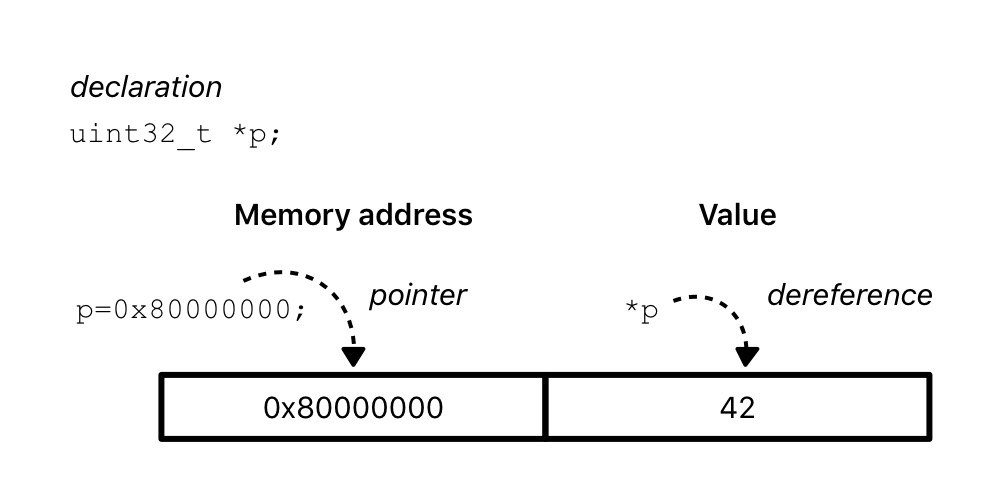
\includegraphics[width=0.6\textwidth]{pointer.jpg}}
\caption{Pointer declaration}
\label{PointerImg}
\end{figure}

Figure \ref{PointerImg} shows a declaration of a variable \textit{p} as a pointer. \textit{p} points to a value of type \textit{uint32\_t}. The pointer is shown to be assigned the memory address 0x80000000. To access the value 42 the variable \textit{p} is dereferenced using \textit{*p}. 

\begin{lstlisting}[language=C,showstringspaces=false,caption={File: swap.c, part 1 swap function},captionpos=b,label=swap]

 1 #include <stdio.h>
 2 #include <assert.h>
 3 #include <stdint.h>
 4 
 5 void swap (uint32_t *a,uint32_t *b)
 6 {
 7 uint32_t tmp;
 8 
 9 assert ((a!=NULL)&&(b!=NULL));
10   if (a==b) return;
11 
12 tmp = *a;
13 *a = *b;
14 *b = tmp;
15 }
 
\end{lstlisting}

Listing \ref{swap} shows the function \textit{swap(...)} function. It takes two pointers of type \textit{uint32\_t} called \textit{*a} and \textit{*b} respectively. The variables are checked to see whether they are non-NULL, see line:9. If either variable is NULL then the program will terminate. Line:10 checks to see if the pointers point to the same memory address. If so then there is no requirement to do the swap. Lines:12-14 carries out the swap mechanism, swapping the values in the locations of \textit{a} and \textit{b} in memory.

\subsection{Reference pointers}
 
\index{pointers!references}
 
A \textit{reference} is symbolized by the character \& i.e.  \&\textless{variable name}\textgreater. A reference variable is fixed to a specific address, it cannot be used in an arithmetic calculation and can only be assigned at initialization time.

\begin{figure}[H]
\centerline{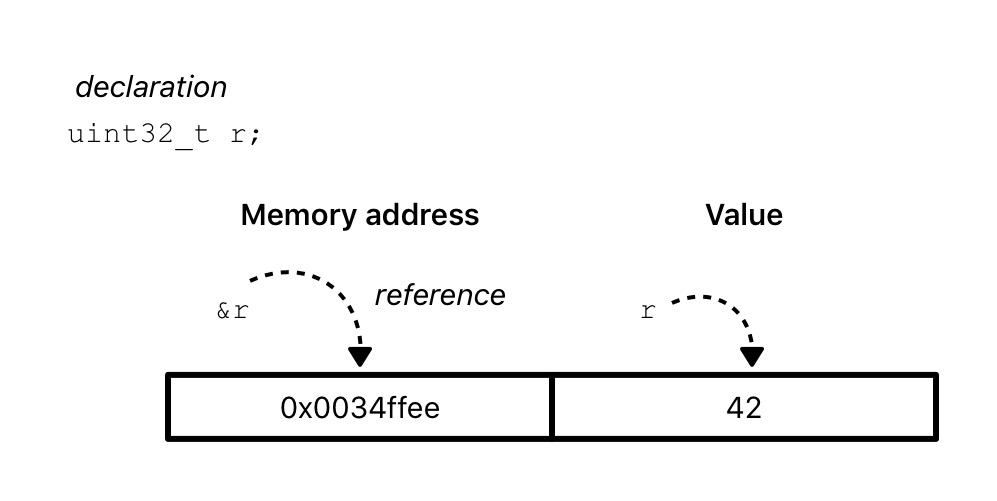
\includegraphics[width=0.6\textwidth]{reference.jpg}}
\caption{Reference declaration}
\label{ReferenceImg}
\end{figure}

Figure \ref{ReferenceImg} shows a declaration of a variable \textit{r} of type \textit{uint32\_t}. To obtain the memory address or reference pointer for \textit{r}, \&\textit{r} is used. In the figure, the reference pointer is memory address 0x0034ffee. To access the value 42 the variable \textit{r} is simply used. This reference pointer is fixed by the compiler at build time. 
   
\begin{lstlisting}[language=C,showstringspaces=false,caption={File: swap.c, part 2},captionpos=b,label=reference]

18 int main(void)
19 {
20 uint32_t x=10,y=20;
21 
22 printf("...start swap\n");
23 printf(" x memory address : 0x%08x\n",(uint32_t)&x);
24 printf(" y memory address : 0x%08x\n",(uint32_t)&y);
25 
26 printf("... init: x=%d,y=%d\n",x,y);
27 
28 swap(&x,&y);
29 printf("... swap: x=%d,y=%d\n",x,y);
30 
31 swap(&x,&y);
32 printf("... swap: x=%d,y=%d\n",x,y);
33 
34 return 0;
35 }

INTERACTION

$ cc swap.c
$ ./a.out
...start swap
 x memory address : 0x5666fba8
 y memory address : 0x5666fba4
... init: x=10,y=20
... swap: x=20,y=10
... swap: x=10,y=20
$
\end{lstlisting}

The listing \ref{reference} shows how references and pointers interact. The example shows a double swap of the variables \textit{x} and \textit{y}. Lines:23:24 prints out the memory address assigned to the variables. The memory addresses never change throughout but the data will change. The variables will have the same value at the start and end of the program. The variables are passed as references into the \textit{swap(...)} function. 

\subsection{void *}

\index{pointers!void pointers}

As discussed in section \ref{voidtype}, \textit{void *} is a generic pointer to any object. It is used to build structures of different types. \textit{void *} does not point to a specific type with a particular size. It is useful for building generic functions that cover multiple different datatypes. 

\subsection{Function pointer}

\index{pointers!function pointer}

The function pointer concept is a powerful feature in the C Programming Language. It allows a function to be a variable. This means that a function can be passed in as a parameter, as well as being placed in a table or structure. We will discuss the table and structure concept in more detail in section \ref{datastructure}.
 
\begin{lstlisting}[language=C,caption={Function Pointer Syntax},captionpos=b,label=functpointer]

<return-type> (*<function pointer name>)({<parameter-list>})

\end{lstlisting}

Listing \ref{functpointer} shows the syntax of a function pointer. The function pointer has a \textit{return-type} similar to a normal function. The brackets ( ... ) along with the *\textless{function pointer name}\textgreater \, identify a function pointer. The \textit{parameter-list} is the same as a standard function definition. 

\begin{lstlisting}[language=C,showstringspaces=false,caption={File: funpointer.c},captionpos=b,label=funpointer]

 1 #include <stdio.h>
 2 #include <math.h>
 3 
 4 double calculate45degrees(double (*funct)(double))
 5 {
 6 return funct(45.0);
 7 }
 8 
 9 int main(void)
10 {
11 printf ("sin(45.0) = %lf\n",calculate45degrees(sin));
12 printf ("cos(45.0) = %lf\n",calculate45degrees(cos));
13 
14 return 0;
15 }

INTERACTION

$ cc funpointer.c
$ ./a.out
sin(45.0) = 0.850904
cos(45.0) = 0.525322
$

\end{lstlisting}


Listing \ref{funpointer} shows an example of a generic function call \textit{calculate45degrees(...)} on lines:4-7. The function has a function pointer parameter called \textit{funct}. In the body of the function the function pointer is called with the value of 45.0. The result of invoking this function is returned to the caller, in this case \textit{main(...)}. 

The caller calls \textit{calculate45degrees(...)} twice with different functions, first the \textit{sin(...)} function and then \textit{cos(...)} function as shown on lines:11:12.


